\documentclass[
	12pt,				% tamanho da fonte
	openright,			% capítulos começam em pág ímpar (insere página vazia caso preciso)
	oneside,			% para impressão em recto e verso. Oposto a oneside
	a4paper,			% tamanho do papel.
    tikz,
	english,			% idioma adicional para hifenização
	french,				% idioma adicional para hifenização
	spanish,			% idioma adicional para hifenização
	brazil				% o último idioma é o principal do documento
	]{abntex2}

% ---
% Pacotes básicos
% ---
\usepackage{lmodern}			% Usa a fonte Latin Modern
\usepackage[T1]{fontenc}		% Selecao de codigos de fonte.
\usepackage[utf8]{inputenc}		% Codificacao do documento (conversão automática dos acentos)
\usepackage{lastpage}			% Usado pela Ficha catalográfica
\usepackage{indentfirst}		% Indenta o primeiro parágrafo de cada seção.
\usepackage{color}				% Controle das cores
\usepackage{graphicx}			% Inclusão de gráficos
\usepackage{microtype} 			% para melhorias de justificação
\usepackage{pgfplots}
\usetikzlibrary{patterns}
% ---

% ---
% Pacotes de citações
% ---
\usepackage[brazilian,hyperpageref]{backref}	 % Paginas com as citações na bibl
\usepackage[alf]{abntex2cite}	% Citações padrão ABNT

\usepackage{lipsum}				% para geração de dummy text

% ---
% Informações de dados para CAPA e FOLHA DE ROSTO
% ---
\titulo{Competências do Engenheiro da Computação em 2030}
\autor{Carlos Antonio Marques Maniero --- 1824312}
\local{UNIVESP}
\data{2018}
\orientador{Prof.\ Dr.\ Maurício B. de Camargo Salles}
\instituicao{%
  Univesidade Virtual do Estado de São Paulo --- UNIVESP
  \par
  Curso de Engenharia da Computação
  \par
  Diciplina de Introdução à Engenharia de Computação --- IEC001
}
\tipotrabalho{Atividade Avaliativa}
% O preambulo deve conter o tipo do trabalho, o objetivo,
% o nome da instituição e a área de concentração
\preambulo{Atividade avaliativa apresentado como
    exigência parcial para Avaliação da Diciplina de
    Introdução à Engenharia de Computação
    do curso de Engenharia da Computação pela UNIVESP.}
% ---


% ---
% Configurações de aparência do PDF final

% alterando o aspecto da cor azul
\definecolor{blue}{RGB}{41,5,195}

% informações do PDF
\makeatletter

\hypersetup{pdftitle={\@title},
            pdfauthor={\@author},
            pdfsubject={\imprimirpreambulo},
            pdfcreator={LaTeX with abnTeX2},
            colorlinks=true,       		% false: boxed links; true: colored links
            linkcolor=blue,          	% color of internal links
            citecolor=blue,        		% color of links to bibliography
            filecolor=magenta,      		% color of file links
            urlcolor=blue,
            bookmarksdepth=4}
\makeatother
% ---

% ---
% Espaçamentos entre linhas e parágrafos
% ---

% O tamanho do parágrafo é dado por:
\setlength{\parindent}{1.3cm}

% Controle do espaçamento entre um parágrafo e outro:
\setlength{\parskip}{0.2cm}  % tente também \onelineskip

% ---
% compila o indice
% ---
\makeindex
% ---

% ----
% Início do documento
% ----
\begin{document}

% Seleciona o idioma do documento (conforme pacotes do babel)
%\selectlanguage{english}
\selectlanguage{brazil}

% Retira espaço extra obsoleto entre as frases.
\frenchspacing

% ----------------------------------------------------------
% ELEMENTOS PRÉ-TEXTUAIS
% ----------------------------------------------------------
% \pretextual

% ---
% Capa
% ---
\imprimircapa{}
% ---

% ---
% Folha de rosto
% (o * indica que haverá a ficha bibliográfica)
% ---
\imprimirfolhaderosto*
% ---

% ---
% Epígrafe
% ---
\begin{epigrafe}
    \vspace*{\fill}
	\begin{flushright}
        \begin{adjustwidth}{7.5cm}{}
        \textit{``Não é a consciência do homem que lhe
            determina o ser, mas, ao contrário,
            o seu ser social que lhe determina a
            consciência.''}
        \end{adjustwidth}
        \textit{Karl Marx}
	\end{flushright}
\end{epigrafe}
% ---

% ---
% inserir o sumario
% ---
\pdfbookmark[0]{\contentsname}{toc}
\tableofcontents*
\cleardoublepage{}
% ---

% ----------------------------------------------------------
% ELEMENTOS TEXTUAIS
% ----------------------------------------------------------
\textual{}

% ----------------------------------------------------------
% Introdução (exemplo de capítulo sem numeração, mas presente no Sumário)
% ----------------------------------------------------------
\chapter*[Introdução]{Introdução}
\addcontentsline{toc}{chapter}{INTRODUÇÃO}
É de conhecimento geral de que com a revolução industrial,
o trabalhador teve o produto de seu trabalho exponenciado
com a introdução de maquinários: produto da Engenharia.
O fim das video-locadoras se deu com o surgimento dos DVDs
e teve seu ciclo completo com os serviços de \textit{streaming}
afetando tanto as práticas comerciais quanto as sociais.

\par
A engenharia se reinventa a cada dia e manter-se atualizado
faz parte do trabalho de um engenheiro.

\chapter{Competências técnicas: Um novo modelo de Automação}

A automação sempre foi o cabo chefe da computação. Por sua vez,
o termo computador era originalmente designado à pessoas que
faziam cálculos, isto é, computavam. Essa profissão foi extinta
com o surgimento dos computadores eletrônicos. E esse foi um
esforço histórico da engenharia para criar um recurso automatizado
capaz de fazer cálculos de maneira rápida e precisa.

\par

Uma pesquisa da \hbox{\cite{McKinseyAutomacao}} afirma que 78\% dos
trabalhos manuais previsíveis, são passíveis de automação.

\par

\begin{figure}[htb]\centering
    \begin{minipage}{\textwidth}
        \centering
        \caption{Onde máquinas podem substituir humanos}
        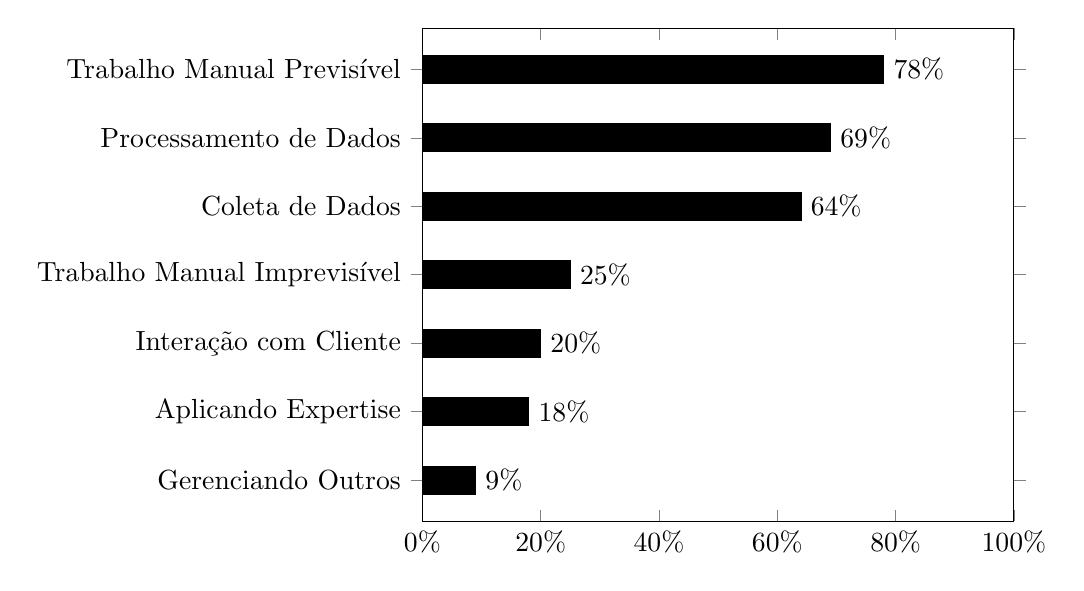
\begin{tikzpicture}
            \begin{axis}[
                xbar,
                width=0.75\textwidth,
                symbolic y coords={Gerenciando Outros,
                    Aplicando Expertise,
                    Interação com Cliente,
                    Trabalho Manual Imprevisível,
                    Coleta de Dados,
                    Processamento de Dados,
                    Trabalho Manual Previsível},
                ytick=data,
                nodes near coords={\pgfmathprintnumber\pgfplotspointmeta\%},
                nodes near coords align={horizontal},
                xmin=0,
                xmax=100,
                xticklabel={\pgfmathparse{\tick}\pgfmathprintnumber{\pgfmathresult}\%},
              ]
                \addplot[draw=black,fill=black] coordinates
                {(9,Gerenciando Outros)
                 (18,Aplicando Expertise)
                 (20,Interação com Cliente)
                 (25,Trabalho Manual Imprevisível)
                 (64,Coleta de Dados)
                 (69,Processamento de Dados)
                 (78,Trabalho Manual Previsível)};
            \end{axis}
        \end{tikzpicture}
        \legend{\cite{McKinseyAutomacao}}
    \end{minipage}
\end{figure}

\section{Machine Learning}

Segundo a pesquisa é imprescindível a utilização de
\textit{Machine Learning} para que a automação de tarefas
com baixo nível de previsibilidade sejam completamente
automatizadas. Está sendo considerado o trabalho conjunto entre
humanos e máquinas, onde as máquinas sejam capazes reconhecer
e aprender padrões com humanos para conseguir atuar mesmo
nos mais imprevisíveis ambientes.

\par
Um dos maiores desafios nesse procedimento é que tenhamos máquinas
capazes de reconhecer de maneira satisfatória a linguagem
natural. Para o engenheiro do futuro, não bastará só compreender
o domínio do negócio e automatiza-lo. O conhecimento sobre
\textit{Machine Learning} será necessário para que a automação
de processos seja possível utilizando máquinas que possam exercer o
papel de um humano com o mesmo grau de precisão, mesmo nos mais
imprevisíveis ambientes.

\chapter{O futuro é comportamental!}

O trabalho do engenheiro não é mais como antigamente. Quando
falamos de um projeto de engenharia, não estamos mais falando
sobre um engenheiro, debruçado sobre uma mesa com uma calculadora
HP e um lápis projetando alguma coisa no papel.

\par

Quando falamos de engenheiros, estamos falando de equipes
multidisciplinares e diversas. Para tal, o engenheiro precisa
estar preparado para o desafio além do técnico. O desenho
técnico agora é digital. É possível simular toda a manufatura
de uma empresa com um simples clique. O trabalho do engenheiro
mudou.

Segundo a \hbox{\cite{WeForum}} 35\% das competências que eram
consideradas importantes para qualquer profissional em 2015
mudaram de prioridade 2020. E com a quarta revolução industrial,
teremos acesso à robótica avançada, transporte autônomo,
inteligência artificial, biotecnologia e genômica.


\begin{table}[htb]
\ABNTEXfontereduzida{}
\caption{Competências desejadas em 2015}
\begin{tabular}{p{0.1\textwidth}|p{0.9\textwidth}}
   \textbf{Posição} & \textbf{Competência} \\
    \hline
    1 & Resolução de problemas complexos \\
    \hline
    2 & Coordenar com outros \\
    \hline
    3 & Gerenciamento de pessoas \\
    \hline
    4 & Pensamento crítico \\
    \hline
    5 & Negociação \\
    \hline
    6 & Controle de Qualidade \\
    \hline
    7 & Operação orientada a serviços \\
    \hline
    8 & Julgamento e tomada de decisões \\
    \hline
    9 & Escuta ativa \\
    \hline
    10 & Criatividade \\
\end{tabular}
\end{table}

\begin{table}[htb]
\ABNTEXfontereduzida{}
\caption{Competências desejadas em 2020}
\begin{tabular}{p{0.1\textwidth}|p{0.9\textwidth}}
   \textbf{Posição} & \textbf{Competência} \\
    \hline
    1 & Resolução de problemas complexos \\
    \hline
    2 & Pensamento crítico \\
    \hline
    3 & Criatividade \\
    \hline
    4 & Gerenciamento de pessoas \\
    \hline
    5 & Coordenar com outros \\
    \hline
    6 & Inteligência emocional \\
    \hline
    7 & Julgamento e tomada de decisões \\
    \hline
    8 & Operação orientada a serviços \\
    \hline
    9 & Negociação \\
    \hline
    10 & Flexibilidade Cognitiva \\
\end{tabular}
\end{table}

\chapter{Conclusão}

A engenharia vem passando por um processo de democratização.
Isso se iniciou com o surgimento do conceito de código aberto.
Hoje, mais do que \textit{software}, temos \textit{hardware} aberto,
por exemplo, o Arduino. Com isso, vemos um grupo mais diverso
de engenheiros no mercado.

\par

Com a automatização de processos, novas tecnologias e
\textit{frameworks}. Deixamos de ter os engenheiros à serviço
da tecnologia e passamos a ter a tecnologia a serviço dos
engenheiros. Com isso, os engenheiros podem focar no que mais
importa: resolver problemas. Mais do que excelência
técnica é necessário que o engenheiro desenvolva-se na área
de competências comportamentais.

\par
O futuro está próximo, e temos cada vez mais ferramentas a disposição
dos engenheiros. Comandos por voz e máquinas que aprendem sozinhas
já é uma realidade e desenvolver-se nessas áreas é importantíssimo.

% ----------------------------------------------------------
% Referências bibliográficas
% ----------------------------------------------------------
\bibliography{introducao-a-engenharia-da-computacao-semana-4}

\end{document}
